\section{Modello Computazionale}
Il modello computazionale consiste in un programma di simulazione di tipo
next-event che impiega il metodo ``batch means'' per il calcolo di tutte le
metriche di interesse. 
A questo livello di astrazione del sistema si passa ad implementare tutto ciò
che è stato definito formalmente nel modello di specifica, in particolare in
questa sezione verranno descritte le strutture dati impiegate per la
rappresentazione delle variabili, le funzioni ed i costrutti che realizzano la
logica del sistema, come vengono generati i dati di input alla simulazione ed
infine le metodologie con cui vengono collezionati ed elaborati i dati di
output.

La simulazione viene eseguita un numero R di
volte in modo da ottenere un campione di tale dimensione con cui generare un
intervallo di confidenza al 95\% per le statistiche ottenute.  Le replicazioni
della simulazione sono gestite con un ciclo for all’inizio del quale vengono
re-inizializzate tutte le variabili e viene reimpostato il seme per il PRNG
affinché le distribuzioni generate in ogni replicazione siano indipendenti. In
ogni replicazione i valori delle variabili vengono scritti in modo iterativo su
dei file di output che vengono poi elaborati tramite un successivo programma per
il calcolo delle metriche di interesse.
%
%
\subsection{Strutture Dati}
In primo luogo, vengono definite le strutture dati riguardanti la lista degli
eventi possibili ed il clock che regola il tempo di simulazione, successivamente
quelle che contegono i dati di output ed infine la struttura dati relativa alla
principale entità manipolata nel sistema: i task (job).
%
\subsubsection{Eventi e Clock Virtuale}
Ad ogni istante la lista di eventi è così composta:
\begin{itemize}
\item[-]prossimo arrivo job di classe 1
\item[-]prossimo arrivo job di classe 2
\item[-]al più $N$ completamenti di job nel cloudlet
\item[-]$0$ o più completamenti di job nel cloud
\item[-]$0$ o più completamenti di fase di setup dei job interrotti
\end{itemize}
non essendovi un numero finito di eventi da gestire, occorre realizzare la lista
di eventi tramite una struttura dati dinamica, pertanto gli eventi vengono
gestiti tramite una coda prioritaria, ordinata per scadenza, ovvero con una
politica del tipo Least Remaining Time (figura~\ref{eventq}).
%
\begin{figure}[!h]
\centering
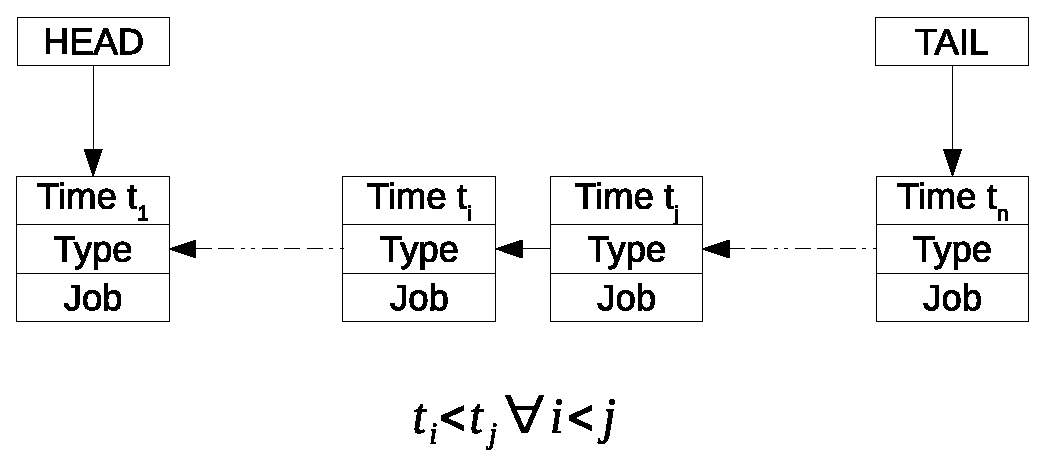
\includegraphics[width=0.7\textwidth]{figures/eventq}
\caption{Coda prioritaria di eventi, ordinata per istante di scadenza}
\label{eventq}
\end{figure}
%
\\Un generico evento è composto dai seguenti campi:
\begin{itemize}
\item L’istante in cui l’evento si verifica
\item La tipologia di evento (arrivo, partenza, setup)
\item Il job associato
\item Un array contenente lo stato del sistema (la sua struttura verrà discussa
più avanti)
\end{itemize}

Ogniqualvolta viene creato un evento, questo viene inserito nella coda nella
posizione opportuna tramite un’operazione di \emph{enqueue}, affinché ogni 
operazione di \emph{dequeue} estragga l’evento più imminente.

Il tempo di simulazione è regolato da un clock virtuale che tiene conto
dell’istante corrente e del successivo in modo tale da poter considerare
intervalli di tempo utili per il calcolo di statistiche di tipo time-averaged.

\begin{figure}[!h]
\begin{lstlisting}[title=basic.h]
struct event {
    double time;
    struct job_t job;
    unsigned int type;
    unsigned int n[4];
};

typedef struct {           /* simulation clock                  */
    double current;        /*   current time                    */
    double next;           /*   next (most imminent) event time */
} clock;
\end{lstlisting}
\end{figure}

%
\subsubsection{Variabili di Output}
I dati che man mano devono essere raccolti durante la simulazione sono
memorizzati in variabili suddivise in base alla tipologia e al nodo di
esecuzione dei job. Per esempio, lo stato del sistema, così come il numero di
arrivi e completamenti, è implementato tramite un array di dimensione 4, di cui
ogni slot corrisponde ad una combinazione classe-nodo a cui il job può essere
associato. 

L’accesso ad uno slot dell’array viene effettuato tramite un indice
che viene calcolato tramite la somma di macro che rappresentano le varie
combinazioni, infatti, se si vuole considerare il numero di job di classe 1 in
esecuzione nel cloud basta accedere all’array tramite l’indice che deriva dalla
somma delle macro J\_CLASS1 e CLOUD. La tabella X descrive le possibili
combinazioni di macro legate all’indice di accesso.

[TABELLA X]

%
\subsubsection{Task}
Un generico task, anche detto job, viene implementato come una struttura
specifica dotata dei seguenti attributi: 
\begin{itemize}
\item[id]: identificatore univoco necessario ad effettuare un riordino dei job
nel momento in cui vanno considerate le statistiche in un ordine corrispondente
agli istanti di arrivo dei singoli job
\item[class]: specifica la classe del job, può assumere il valori J\_CLASS1 e
J\_CLASS2 (macro definite nel file di configurazione); 
\item[node]: specifica il nodo in cui il job è in esecuzione, può assumere i
valori CLET, CLOUD, SETUP (macro definite nel file di configurazione), che
corrispondono rispettivamente a cloudlet, cloud e nodo di setup; 
\item[service]: array che memorizza i tempi di risposta seguendo la stessa regola
delle combinazioni che riguarda anche lo stato del sistema. Un job di classe 1
in esecuzione nel cloud avrà un tempo di risposta non nullo nello slot relativo,
un job interrotto avrà un tempo di risposta non nullo sia nello slot riguardante
il nodo cloudlet che in quello riguardante il nodo cloud.  setup: tempo che un
job trascorre in fase di setup. Il valore rimane nullo nel caso in cui il job
non viene interrotto.  
\end{itemize}
\begin{figure}[!h]
\begin{lstlisting}[title=basic.h]
struct job_t {
    unsigned long id;
    unsigned int class;
    unsigned int node;
    double service[4];
    double setup;
};
\end{lstlisting}
\end{figure}
%
%
\subsection{Generazione dell'input}
I dati di input della simulazione, corrispondenti ai tempi di interarrivo e di
servizio dei singoli job, vengono generati a runtime in base alle informazioni
note sulle relative distribuzioni esponenziali. Per ottenere tali distribuzioni
sono state utilizzate le funzioni delle librerie rvgs e rngs di \emph{Steve
Park} e \emph{Dave Geyer} descritte in \cite{leemis}.

La funzione \emph{GetArrival()}, ogniqualvolta viene chiamata, restituisce il
più imminente istante di arrivo tra un job di classe 1 ed uno di classe 2 e
memorizza nella variabile j, passata per riferimento, la classe del job in
questione. Tali istanti di arrivo vengono calcolati progressivamente a seguito
della generazione dei tempi di interarrivo tra un job e l’altro, più
precisamente, non appena viene restituito un istante di arrivo relativo al job
di una classe, viene calcolato il successivo per la medesima classe.

La funzione \emph{GetService()} restituisce un valore che deriva dalla
generazione di un tempo di servizio esponenziale con media stabilita in base ai
parametri j e n passati come argomento che indicano rispettivamente la classe ed
il nodo di esecuzione del job.

La funzione \emph{GetSetup()} restituisce semplicemente un valore generato a
partire da una distribuzione esponenziale di media $E[S_{setup}]$.

Le funzioni in questione sono elencate di seguito. Si noti che prima di ogni
chiamata alle funzioni della libreria \emph{rvgs} viene selezionato, tramite la
funzione \emph{SelectStream()}, un flusso di generazione di numeri
pseudo-casuali distinto, affinché sia garantita il più possibile l’indipendenza
tra le sequenze di numeri generate.  
%
%
